\section{Irreduzibilitätstest nach Rabin}

Der in \autoref{sec:berlekamp} vorgestellte Algorithmus von Berlekamp
faktorisiert (quadratfreie) Polynome stets vollständig. Jedoch kann man sich
Anwendungen vorstellen, in denen lediglich interessant ist, ob ein Polynom
irreduzibel ist oder nicht. Dabei würde eine Anwendungen des
Berlekamp-Algorithmus unnötige Arbeit leisten. 
Daher wollen wir das zentrale Resultat von \citeauthor{rabin} aus 
\autocite{rabin} zitieren, das den gleichnamigen Algorithmus motiviert.

\begin{thm}
  \label{satz:rabin}
  Sei $f(X) \in \F_q[X]$ monisch von Grad $n$. Seien $p_1,\ldots,p_k$ alle
  paarweise verschiedenen Primteiler von $n$. Notiere mit $n_i$ den Kofaktor
  von $p_i$ in $n$, also $n_i := \tfrac{n}{p_i}$ für $i=1,\ldots,k$. Dann gilt:
  $f(X)$ ist irreduzibel über $\F_q$ genau dann, wenn
  \begin{enumerate}
    \item $f(X) \mid (X^{q^n}-X)$,
    \item $\ggT(g(X), X^{q^{n_i}}-X) = 1$ für alle $i=1,\ldots,k$.
  \end{enumerate}
\end{thm}
\begin{proof}
  \autocite[Lemma 1]{rabin}. Dort zwar nur für $\Z_p$, jedoch lässt sich der
  Beweis für beliebiges $\F_q$ problemlos erweitern.
\end{proof}

Damit ist klar, wie man mit \thref{satz:rabin} einen Irreduzibilitätstest
gestaltet. Es gilt lediglich zu bemerken, dass die Berechnung des 
$\ggT(g(X),X^{q^n_i}-X)$ in dieser Form aufgrund des hohen Grades des zweiten
Polynoms sehr schwierig wäre. Daher erfolgt zuvor eine Reduktion von
$X^{q^{n_i}}-X \bmod f(X)$.

\haskellinput{Algorithmen/Rabin}{rabin}

Zu beachten gilt, dass die Reduktion $\bmod f(X)$ nicht mit dem in
\autoref{sec:polynomials} vorgestellten ħmodByPħ durchgeführt wird, sondern
eine separate Funktion implementiert wurde, die effizient durch einen
\emph{Divide-And-Conquer}-Ansatz $X^{q^{n_i}} \bmod f(X)$ berechnet.

\haskellinput{Algorithmen/Rabin}{modMonom}

Die Zerlegung von $n$ in seine Primfaktoren wird durch ħnub . factorħ
bewerkstelligt, wobei ħnubħ aus ħData.Listħ Duplikate in Listen entfernt.
ħfactorħ ist gegeben durch:

\haskellinput{Algorithmen/Rabin}{factor}

\subsection{Ein kleiner Vergleich}

Auch wenn der Vergleich einer vollständigen Faktorisierung via Berlekamp mit
Rabin als Irreduzibilätstest ob des Mehraufwands nicht ganz fair ist, so wollen
wir ihn doch anführen. \autoref{fig:berlevsrabin} deutlich, dass die bloße Information der
Irreduzibilität viel leichter zu gewinnen ist, als die gesamte Faktorisierung.
(Wer hätte das gedacht!)

\begin{figure}
  \caption{Vergleich Berlekamp vs Rabin als Irreduzibilitätstest}
  \label{fig:berlevsrabin}
  \centering
  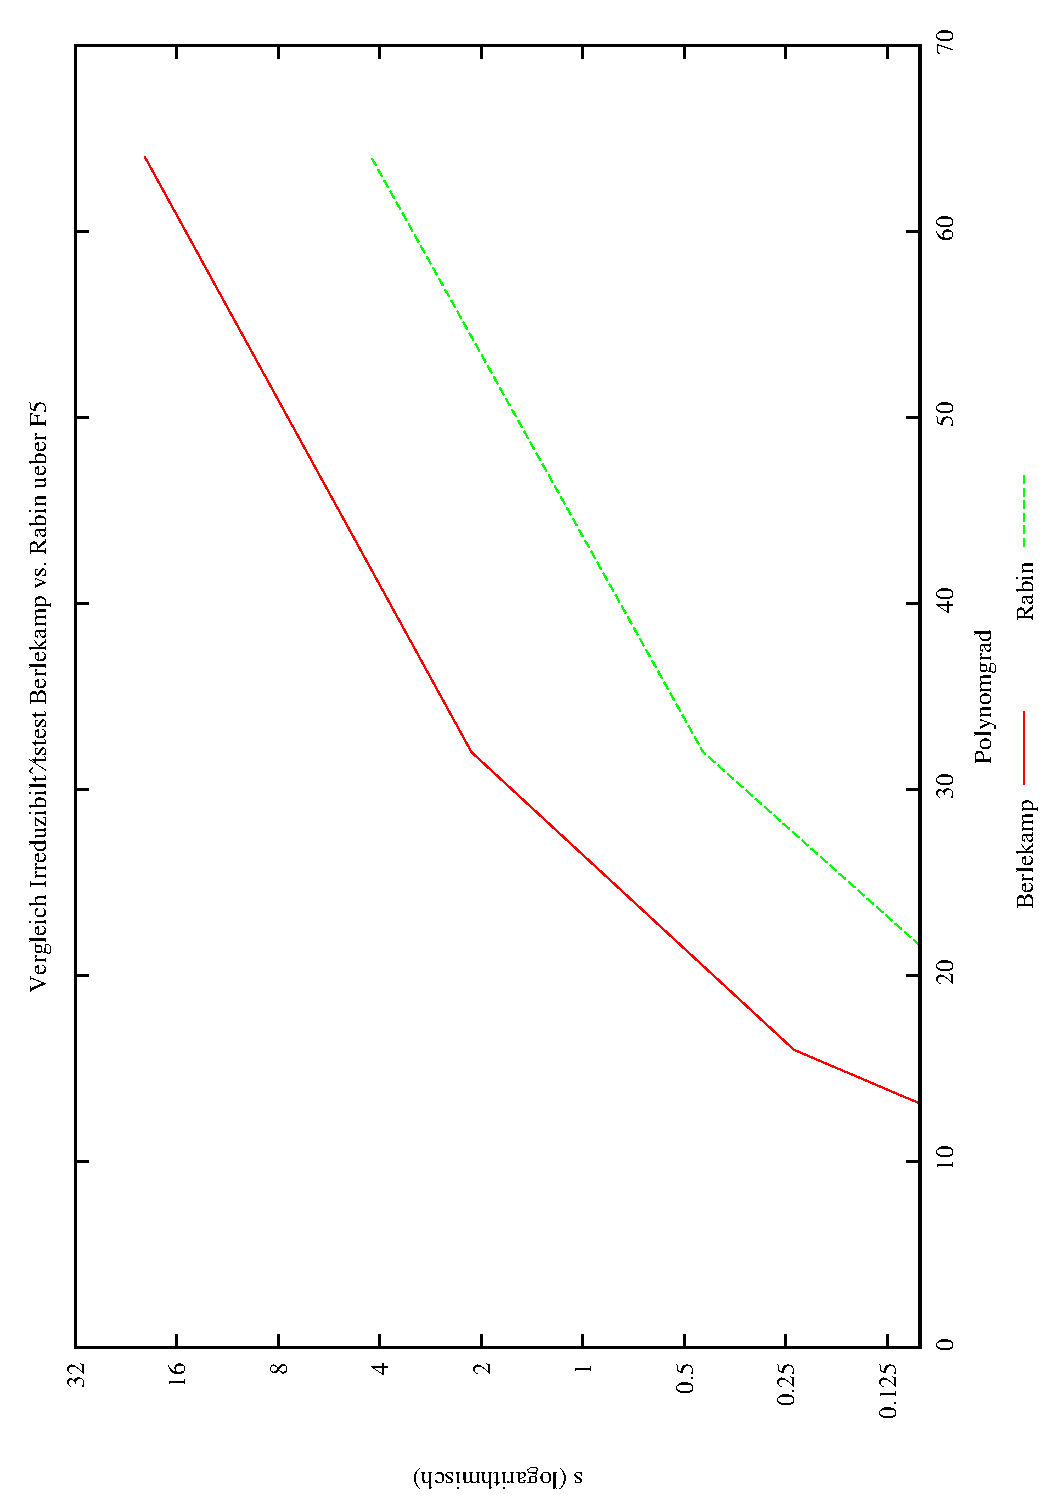
\includegraphics[angle=-90,width=0.7\textwidth]{plots/benchBerleVsRabin_F5.pdf}
  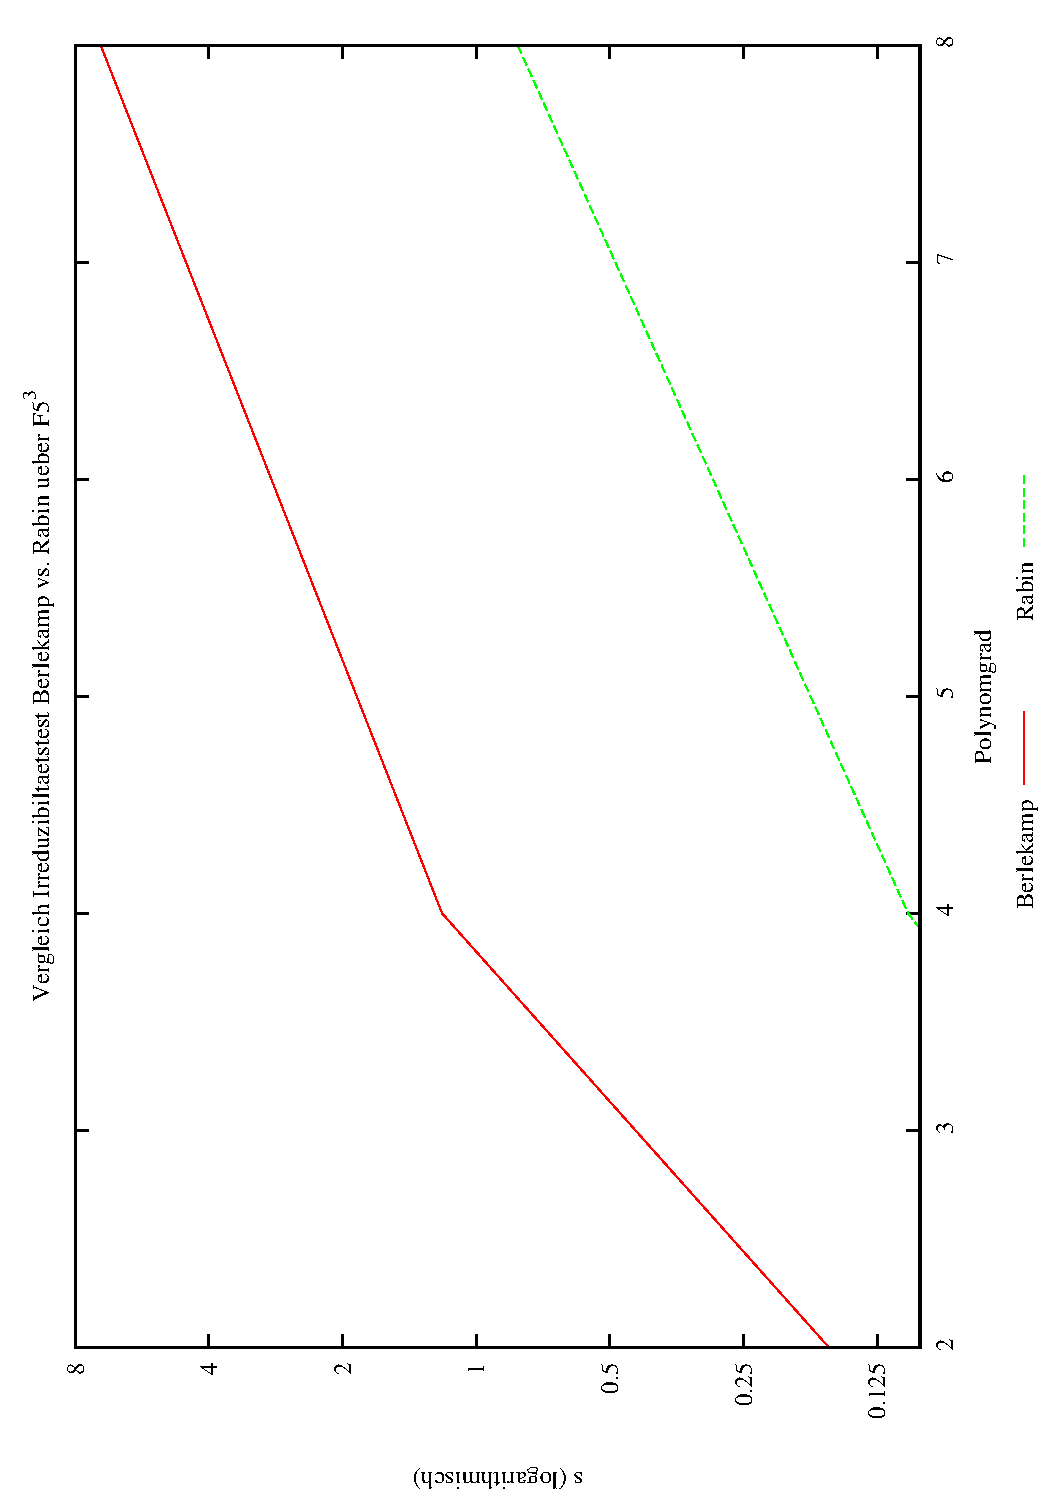
\includegraphics[angle=-90,width=0.7\textwidth]{plots/benchBerleVsRabin_F53.pdf}
\end{figure}
